% \chapter{Path Planning}\label{chap:pathplanning}
\chapter{路径规划}
\label{chap:pathplanning}
% Path-planning is an important primitive for autonomous mobile robots that lets robots find the shortest---or otherwise optimal---path between two points. Optimal paths could be paths that minimize the amount of turning, the amount of braking or whatever a specific application requires. Algorithms to find a shortest path are important not only in robotics, but also in network routing, video games and understanding protein folding.

路径规划是自主移动机器人的重要原语,让机器人找到两点之间最短或最佳的路径。最佳路径可以是最小化转向、制动或特定应用所需要的路径。寻找最短路径的算法不仅对机器人技术,而且对网络路由、视频游戏和理解蛋白质折叠都很重要。

% Path-planning requires a map of the environment and the robot to be aware of its location with respect to the map. We will assume for now that the robot is able to localize itself, is equipped with a map, and capable of avoiding temporary obstacles on its way. How to create a map, how to localize a robot, and how to deal with uncertain position information will be major foci of the reminder of this  book. The goals of this chapter are to

路径规划需要环境和机器人的地图来了解其相对于地图的位置。我们现在假设机器人能够定位自己,配有地图,并能够避免临时障碍物。如何创建地图、如何定位机器人,以及如何处理不确定的位置信息将是本书剩下部分的主要焦点。本章的目标是

\begin{itemize}
% \item introduce suitable map representations,
% \item explain basic path-planning algorithms  ranging from Dijkstra, to A*, D* and RRT,
% \item introduce variations of the path-planning problem, such as coverage path planning.

\item 介绍合适的地图表示
\item 介绍从Dijkstra到A*,D*和RRT的基本路径规划算法
\item 介绍路径规划问题的变种,如覆盖路径规划
\end{itemize}

% \section{Map representations}\label{sec:maps}
\section{地图表示}
\label{sec:maps}

% In order to plan a path, we somehow need to represent the environment in the computer. We differentiate between two complementary approaches: discrete and continuous approximations. In a discrete approximation, a map is sub-divided into chunks of equal (e.g., a grid or hexagonal map) or differing sizes (e.g., rooms in a building). The latter maps are also known as \emph{topological maps}.\index{Topological map} Discrete maps lend themselves well to a graph representation. Here, every chunk of the map corresponds to a vertex (also known as ``node''), which are connected by edges, if a robot can navigate from one vertex to the other. For example a road-map is a topological map, with intersections as vertices and roads as edges, labeled with their length (Figure \ref{fig:pathproblem}). Computationally, a graph might be stored as an adjacency or incidence list/matrix. A continuous approximation requires the definition of inner (obstacles) and outer boundaries, typically in the form of a polygon, whereas paths can be encoded as sequences of points defined by real numbers. Despite the memory advantages of a continuous representation, discrete maps are the dominant representation in robotics.

为了规划路径,我们需要在计算机中表示环境。我们区分两种互补的方法:离散近似和连续近似。在离散近似中,地图被细分成相同(例如,网格或六边形地图)或不同大小(例如,建筑物中的房间)的块。后者的地图也称为\emph{拓扑图(Topological map)}\index{拓扑图(Topological map)}。离散地图很适用于图形表示。这里,如果机器人可以从一个点导航到另一个点,那么地图的每个块对应于通过边缘连接的点(也称为“节点”)。例如,路线图是一个拓扑图,其中交叉点作为顶点和道路作为边缘,以其长度标注(图\ref{fig:pathproblem})。在计算上,图形可能存储为邻接或入口列表/矩阵。连续近似需要内部(障碍物)和外部边界的定义,通常以多边形的形式,而路径可以被编码为由实数定义的点的序列。尽管连续表现的记忆优势,离散地图是机器人技术中的主要代表。

% For mapping obstacles, the most common map is the \emph{occupancy grid} map\index{Occupancy grid}. In a grid map, the environment is discretized into squares of arbitrary resolution, e.g. 1cm x 1cm, on which obstacles are marked. In a probabilistic occupancy grid, grid cells can also be marked with the probability that they contain an obstacle. This is particularly important when the position of the robot that senses an obstacle is uncertain. Disadvantages of grid maps are their large memory requirements as well as computational time to traverse data structures with large numbers of vertices. A solution to this is storing the grid map as \emph{k-d tree}.\index{k-d tree (data structure)} A k-d tree recursively breaks the environment into $k$ pieces. For $k=4$, an area is broken into four pieces. Each of these pieces is again broken into four pieces and so on, until the desired resolution is reached. These pieces can easily be stored in a graph with each vertex having four children, which are the four pieces the vertex is broken into, or is a leaf of the tree. What makes this data structure attractive is that not all vertices need to be broken down to the smallest possible resolution. Instead only areas, which contain obstacles need to be further broken down. A grid map containing obstacles and the corresponding k-d tree, here a quadtree, are shown in Figure \ref{fig:gridvskdtree}. There is no silver bullet, and each application might require a different solution that could be a combination of different map types.

为了映射障碍,最常见的映射是\emph {占用网格} map \index{占用网格}。在网格图中,将环境离散成任意分辨率的平方,例如。 1cm x 1cm,其上标有障碍物。在概率占用网格中,网格单元也可以以它们包含障碍物的概率来标记。当感知障碍物的机器人的位置不确定时,这是特别重要的。网格图的缺点是它们的大内存需求以及遍历具有大量顶点的数据结构的计算时间。解决方案是将网格图存储为\emph {k-d tree}。\index{k-d tree(data structure)}一个k-d树将环境递归地分解成$ k $个块。对于$ k = 4 $,一个区域分为四个部分。这些片中的每一个再次分成四个等等,直到达到所需的分辨率。这些片段可以容易地存储在每个顶点有四个孩子的图形中,这四个小节是顶点被分解的四个部分,也可以是树的叶子。使数据结构具有吸引力的是,不是所有的顶点都需要分解成最小的分辨率。相反,只有包含障碍的区域需要进一步细分。包含障碍物的网格图和相应的k-d树,这里是四叉树,如图\ref{fig:gridvskdtree}所示。没有银弹,每个应用程序可能需要一个不同的解决方案,可以是不同的地图类型的组合。


\begin{figure}
\centering
\includegraphics[width=\textwidth]{figs/gridvskdtree.png}
% \caption{A grid map and its corresponding quadtree (k-d tree).\label{fig:gridvskdtree}}
\caption{网格图及其对应的四叉树(k-d树).}
\label{fig:gridvskdtree}
\end{figure}


% There exist also every possible combination of discrete and continuous representation. For example, roadmaps for GPS systems are stored as topological maps that store the GPS coordinates of every vertex, but might also contain overlays of aerial and street photography or even 3D point clouds stored in a 8-d tree, also known as a \emph{Octree}\index{Octree}. These different maps are then used at different stages of the path planning stage. 

还存在离散和连续表示的每一种可能的组合。例如,GPS系统的路线图存储为存储每个顶点的GPS坐标的拓扑图,但也可能包含存储在8-d树中的空中和街道摄影或甚至3D点云的叠加层,也称为\emph{八叉树} \index{八叉树}。然后将这些不同的地图用于路径规划阶段的不同阶段。


% \section{Path-Planning Algorithms}
% The problem to find a ``shortest'' path from one vertex to another through a connected graph is of interest in multiple domains, most prominently in the internet, where it is used to find an optimal route for a data packet. The term ``shortest'' refers here to the minimum cumulative edge cost, which could be physical distance (in a robotic application), delay (in a networking application) or any other metric that is important for a specific application. An example graph with arbitrary edge-lengths is shown in Figure \ref{fig:pathproblem}. 

\section{路径规划算法}
通过连接图从一个顶点到另一个顶点找到“最短”路径的问题在多个域中是最为引人注目的,最重要的是在互联网中,用于为数据包找到最佳路由。术语“最短”这里指的是最小累积边缘成本,这可能是物理距离(在机器人应用中),延迟(在联网应用中)或对于特定应用很重要的任何其他度量。 具有任意边长的示例图如图\ref{fig:pathproblem}所示。

\begin{figure}[!htb]
\centering
\includegraphics[width=0.6\textwidth]{figs/dijkstra}
% \caption{A generic path planning problem from vertex I to vertex VI. The shortest path is I-II-III-V-VI with length 13. 
\caption{从顶点I到顶点VI的通用路径规划问题。 最短路径为I-II-III-V-VI,长度为13。} 
\label{fig:pathproblem}
\end{figure}

% \subsection{Robot embodiment}
\subsection{机器人实施}
% In order to deal with the physical embodiment of the robot, which complicates the path-planning process, the robot is reduced to a point-mass and all the obstacles in the environment are grown by half of the longest extension of the robot from its center. This representation is known as configuration space \index{Configuration space}as it reduces the representation of the robot to its $x$ and $y$ coordinates in the plane. An example is shown in Figure \ref{fig:cspace}. The configuration space can now either be used as a basis for a grid map or a continuous representation. 

为了处理机器人的物理实施方案,这使得路径规划过程复杂化,机器人被减少到点质量,并且环境中的所有障碍物都以机器人的最长延伸的一半从其中心生长。 这种表示形式被称为配置空间\index {配置空间},因为它将机器人的表示减少到飞机上的$ x $和$ y $坐标。 一个例子如图\ref{fig:cspace}所示。配置空间现在可以被用作网格图或连续表示的基础。

\begin{figure}[!htb]
\centering
\includegraphics[width=0.9\textwidth]{figs/configurationspace}
% \caption{A map with obstacles and its representation in configuration space, which can be obtained by growing each obstacle by the robot's extension. \label{fig:cspace}}
\caption{具有障碍物的地图及其在配置空间中的表示,可以通过机器人的扩展来增加每个障碍物来获得。 \label{fig:cspace}}
\end{figure}


% \subsection{Dijkstra's algorithm}\index{Dijkstra's Shortest Path Algorithm}
\subsection{Dijkstra算法}\index{Dijkstra's Shortest Path Algorithm}
% One of the earliest and simplest algorithms is Dijkstra's algorithm \cite{dijkstra1959note}. Starting from the initial vertex where the path should start, the algorithm marks all direct neighbors of the initial vertex with the cost to get there. It then proceeds from the vertex with the lowest cost to all of its adjacent vertices and marks them with the cost to get to them via itself if this cost is lower. Once all neighbors of a vertex have been checked, the algorithm proceeds to the vertex with the next lowest cost. Once the algorithm reaches the goal vertex, it terminates and the robot can follow the edges pointing towards the lowest edge cost.

最早和最简单的算法之一是Dijkstra的算法\cite{dijkstra1959note}。从路径应该开始的初始顶点开始,该算法以初始顶点的所有直接邻居标记,其成本达到。然后,从最低成本的顶点到其所有相邻的顶点,然后以成本较低的方式,以自己的成本来标记它们。一旦顶点的所有邻居都已经被检查,则算法以下一个最低的成本进行到顶点。一旦算法到达目标顶点,它终止,机器人可以跟随指向最低边缘成本的边缘。

% In Figure \ref{fig:pathproblem}, Dijkstra would first mark nodes II, III and IV with cost 3, 5 and 7 respectively. It would then continue to explore all edges of node II, which so far has the lowest cost. This would lead to the discovery that node III can actually be reached in $3+1<5$ steps, and node III would be relabeled with cost 4. In order to completely evaluate node II, Dijkstra needs to evaluate the remaining edge before moving on and label node VI with $3+12=15$.

在图\ref{fig:pathproblem}中,Dijkstra将首先标记节点II,III和IV,成本为3,5和7。然后,它将继续探索节点II的所有边缘,该节点目前成本最低。这将导致发现节点III实际上可以以$ 3 + 1 <5 $步长达到,节点III将重新标注成本4.为了完全评估节点II,Dijkstra需要在移动之前评估剩余边缘并标记节点VI $ 3 + 12 = 15 $。

% The node with the lowest cost is now node III (4). We can now relabel node VI with 14, which is smaller than 15, and label node V with $4+5=9$, whereas node IV remains at $4+3=7$. Although we have already found two paths to the goal, one of which better than the other, we cannot stop as there still exist nodes with unexplored edges and overall cost lower than 14. Indeed, continuing to explore from node V leads to a shortest path I-II-III-V-VI of cost 13, with no remaining nodes to explore.

成本最低的节点现在是节点III(4)。我们现在可以重新标记节点VI,其中14个小于15,标签节点V的$ 4 + 5 = 9 $,而节点IV保持在$ 4 + 3 = 7 $。虽然我们已经找到了目标的两条路径,其中一条比另一条更好,但是我们不能停止,因为仍然存在未开发边缘的节点,总成本低于14.实际上,从节点V继续探索导致最短路径I-II-III-V-VI成本13,没有剩余的节点要探索。

% As Dijkstra would not stop until there is no node with lower cost than the current cost to the goal, we can be sure that a shortest path will be found if it exists. We can say that the algorithm is \emph{complete}.\index{Complete (algorithm)}

由于Dijkstra不会停止,直到没有节点成本低于目标的当前成本,我们可以确定如果存在最短路径将被找到。我们可以说算法是\emph {complete}。\index{Complete(algorithm)}

% As Dijkstra will always explore nodes with the least overall cost first, the environment is explored comparably to a wave front originating from the start vertex, eventually arriving at the goal. This is of course highly inefficient in particular if Dijkstra is exploring nodes away from the goal. This can be visualized by adding a couple of nodes to the left of node I in Figure \ref{fig:pathproblem}. Dijkstra will explore all of these nodes until their cost exceeds the lowest found for the goal. This can also be seen when observing Dijkstra's algorithm on a grid, as shown in Figure \ref{fig:dijkstragrid}. 

由于Dijkstra将始终以最小的总体成本来探索节点,因此环境与起始顶点起源的波前相比较,最终达到目标。这当然是非常低效的,特别是如果Dijkstra正在探索远离目标的节点。这可以通过在图\ref{fig:pathproblem}中的节点I的左侧添加几个节点来可视化。 Dijkstra将探索所有这些节点,直到其成本超过目标的最低值。在网格上观察Dijkstra算法时也可以看到,如图\ref{fig:dijkstragrid}所示。

\begin{figure}[htb]
\centering
\includegraphics[width=0.9\textwidth]{figs/dijkstragrid}
% \caption{Dijkstra's algorithm finding a shortest path from `S' to 'G' assuming the robot can only travel laterally (not diagonally) with cost one per grid cell. Note the few number of cells that remain unexplored once the shortest path (grey) is found, as Dijkstra would always consider a cell with the lowest path cost first.\label{fig:dijkstragrid}}
\caption{Dijkstra的算法从“S”到“G”找到最短路径,假设机器人只能以每个网格单元的成本1横向(不是对角线)行进。请注意,一旦发现最短路径(灰色),几何细胞仍然未被探索,因为Dijkstra将始终考虑具有最低路径开销的单元格。 \label{fig:dijkstragrid}}
\end{figure}

% \subsection{A*}\label{sec:astar}\index{A* Shortest Path Algorithm}
\subsection{A*}\label{sec:astar}\index{A* Shortest Path Algorithm}
% Instead of exploring in all directions, knowledge of an approximate direction of the goal could help avoiding exploring nodes that are obviously wrong to a human observer. Such special knowledge that such an observer has can be encoded using a \emph{heuristic function}\index{Heuristic function}, a fancier word for a ``rule of thumb''. For example, we could give priority to nodes that have a lower estimated distance to the goal than others. For this, we would mark every node not only with the actual distance that it took us to get there (as in Dijkstra's algorithm), but also with the estimated cost ``as the crows flies'', for example by calculating the Euclidean distance or the \emph{Manhattan distance}\index{Manhattan distance} between the vertex we are looking at and the goal vertex. This algorithm is known as A* \cite{hart1968formal}. Depending on the environment, A* might accomplish search much faster than Dijkstra's algorithm, and performs the same in the worst case. This is illustrated in Figure \ref{fig:astargrid} using the Manhattan distance metric, which does not allow for diagonal movements. 

知道所有方向的大致方向,而不是探索目标的大致方向,可以帮助避免探索人类观察者明显错误的节点。这样一种观察者可以使用“启发式函数”(“启发式函数”)来进行编码的这种特殊知识,这是一种“经验法则”的爱好者词。例如,我们可以优先考虑与其他目标具有较低估计距离目标的节点。为此,我们将标记每个节点不仅与我们到达那里的实际距离(如在Dijkstra的算法中),而且还与“乌鸦飞行”的估计成本进行比较,例如通过计算欧氏距离或者我们正在看的顶点和目标顶点之间的\emph{Manhattan distance}\index{Manhattan distance}。该算法被称为A * \cite{hart1968formal}。根据环境,A*可能比Dijkstra的算法更快地完成搜索,并且在最坏的情况下执行相同的操作。使用曼哈顿距离度量的图\ref{fig:astargrid}说明,这不允许对角线运动。


\begin{figure}[htb]
\centering
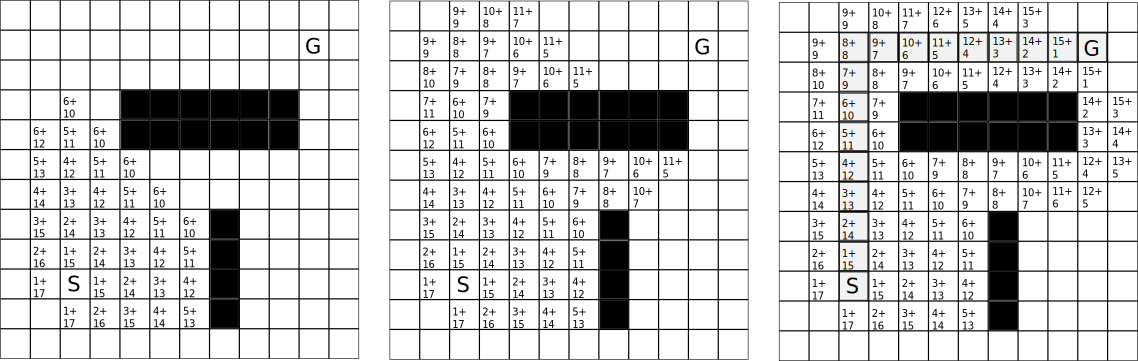
\includegraphics[width=0.9\textwidth]{figs/astargrid}
% \caption{Finding a shortest path from `S' to 'G' assuming the robot can only travel laterally (not diagonally) with cost one per grid cell using the A* algorithm. Much like Dijkstra, A* evaluates only the cell with the lowest cost, but takes an estimate of the remaining distance into account.\label{fig:astargrid}}
\caption{假设机器人只能使用A*算法横向(不对角线)以每个网格单元的成本1来寻找从“S”到“G”的最短路径。很像Dijkstra,A*只评估成本最低的单元格,但考虑到剩余距离的估计。\label{fig:astargrid}}
\end{figure}

% An extension of A* that addresses the problem of expensive re-planning when obstacles appear in the path of the robot, is known as D* \cite{stentz1994optimal}. Unlike A*, D* starts from the goal vertex and has the ability to change the costs of parts of the path that include an obstacle. This allows D* to re-plan around an obstacle while maintaining most of the already calculated path.\index{D*}

A*的扩展解决了当障碍物出现在机器人路径中时昂贵的重新计划的问题,被称为D*\cite{stentz1994optimal}。与A*不同,D*从目标顶点开始,并且具有改变包括障碍物的路径部分成本的能力。这样可以让D*在保持大部分已经计算的路径的同时重新计划障碍物。\index{D*}

% A* and D* become computationally expensive when either the search space is large, e.g., due to a fine-grain resolution required for the task, or the dimensions of the search problem are high, e.g. when planning for an arm with multiple degrees of freedom. Solutions to these problems are provided by sampling-based path planning algorithms that are described further below.

当搜索空间大时,A*和D*在计算上变得昂贵,例如由于任务所需的细粒度分辨率,或者搜索问题的维度高,例如,当规划具有多个自由度的手臂时。这些问题的解决方案是通过以下进一步描述的基于抽样的路径规划算法提供的。

% \section{Sampling-based Path Planning}
\section{基于抽样的路径规划}

% The previous sections have introduced a series of complete algorithms for the path planning problem, i.e. they will find a solution eventually if it exists. Complete solutions are often unfeasible, however, when the possible state space is large. This is the case for robots with multiple degrees of freedom such as arms. In practice, most algorithms are only \emph{resolution complete}\index{Resolution complete}, i.e., only complete if the resolution is fine-grained enough, as the state-space needs to be somewhat discretized for them to operate (e.g., into a grid) and some solutions might be missed as a function of the resolution of the discretization.

前面几节介绍了一系列用于路径规划问题的完整算法,即如果存在,它们将最终找到一个解决方案。然而,当可能的状态空间很大时,完整的解决方案通常是不可行的。对于具有多重自由度的机器人,例如武器就是这种情况。在实践中,大多数算法只有\emph{resolution complete}\index{Resolution complete},即只有在分辨率足够细的情况下才能完成,因为状态空间需要稍微离散化才能运行(例如,进入网格),并且一些解决方案可能被错过作为离散化解决方案的功能。

% Instead of evaluating all possible solutions or using a non-complete Jacobian-based inverse kinematic solution, sampling-based planners create possible paths by randomly adding points to a tree until some solution is found or time expires. As the probability to find a path approaches one when time goes to infinity, sampling-based path planners are \emph{probabilistic complete}\index{Probabilistic complete}. Prominent examples of sampling-based planners are \emph{Rapidly-exploring Random Trees} (RRT)\index{Rapidly-exploring Random Tree}\index{RRT}\cite{lavalle1998rapidly} and \emph{Probabilistic Roadmaps}\index{Probabilistic Roadmaps}\index{PRM}(PRM) \cite{kavraki1996probabilistic}. An example execution of RRT for an unknown goal, thereby reducing the path-planning problem to a search problem is shown in Figure \ref{fig:rrt}.

基于采样的规划者不用评估所有可能的解决方案或使用不完整的基于雅可比的逆运动学解决方案,而是通过将点随机添加到树中创建可能的路径,直到发现某个解决方案或时间到期。当时间到无穷大时,找到路径的概率接近一个,基于抽样的路径规划者是\emph{概率完整的}\index{概率完整}。基于抽样的规划者的突出例子是“快速浏览随机树”(RRT)\index{快速浏览随机树}\index{RRT}\cite{lavalle1998rapidly}和\emph{概率路线图}\index{概率路线图}\index{PRM}(PRM)\cite{kavraki1996probabilistic}。对于未知目标的RRT的示例执行,从而将路径规划问题减少到搜索问题,如图\ref{fig:rrt}所示。

\begin{figure}
\centering
\includegraphics[width=\textwidth]{figs/irrt}
% \caption{Counterclockwise: Random exploration of a 2D search space by randomly sampling points and connecting them to the graph until a feasible path between start and goal is found.\label{fig:rrt}}
\caption{逆时针:通过随机采样点和连接到图形来随机搜索2D搜索空间,直到发现开始和目标之间的可行路径。\label{fig:rrt}}
\end{figure}

% This example illustrates well how a sampling-based planner can quickly explore a large portion of space and refines a solution as time goes on. Whereas RRT can be understood as growing a single tree from a robot's starting point until one of its branches hit a goal, probabilistic road-maps create a tree by randomly sampling points in the state-space, testing whether they are collision-free, connecting them with neighboring points using paths that reflect the kinematics of a robot, and then using classical graph shortest path algorithms to find shortest paths on the resulting structure. The advantage of this approach is clearly that such a probabilistic roadmap has to be created only once (assuming the environment is not changing) and can then be used for multiple queries. PRMs are therefore a \emph{multi-query} path-planning algorithm.\index{Multi-query (path-planning)} In contrast, RRT's are known as \emph{single-query}\index{Single-query (path-planning)} path-planning algorithms.

此示例说明了基于抽样的计划员如何快速探索大部分空间,并随着时间的推移来提炼解决方案。而RRT可以被理解为从机器人的起点生长单个树,直到其一个分支击中目标,概率道路图通过在状态空间中随机采样点来测试它们是否无碰撞,连接它们与相邻点使用反映机器人的运动学的路径,然后使用经典的图最短路径算法来找到最终结构上的最短路径。这种方法的优点是很明显,这样一个概率路线图只能被创建一次(假设环境没有改变),然后可以用于多个查询。PRM因此是一个\emph{multi-query}路径规划算法。\index{多查询(路径规划)}相反,RRT被称为\emph{single-query}\index{Single-query(path计划)}路径规划算法。

% In practice, the boundary between the different historic algorithms has become very diffuse, and single-query and multi-query variants of both RRT and PRM exist. It is important to note that there is no silver bullet algorithm/heuristic and even their parameter-sets are highly problem-specific. We will therefore limit our discussion on useful heuristics that are common to sampling-based planners.

实际上,不同历史算法之间的边界已经变得非常漫长,存在RRT和PRM的单查询和多查询变体。重要的是要注意,没有银色子弹算法/启发式,甚至他们的参数集都是高度针对问题的。因此,我们将限制我们对基于抽样的规划者常见的有用启发式的讨论。


% \subsection{Basic Algorithm}
\subsection{基本算法}
% Let $ \mathcal{X}$ be a $ d$-dimensional state-space. This can either be the robot's state given in terms of translation and rotations (6 dimensions), a subset thereof, or the joint space with one dimension per possible joint angle. Let $ \mathcal{G} \subset \mathcal{X}$ be a  d-ball (d-dimensional sphere) in the state-space that is considered to be the goal, and $ t$ the allowed time. A tree planner proceeds as follows:

让$\mathcal{X}$成为一个$d$维度的状态空间。这可以是根据平移和旋转(6个维度),其子集或者每个可能的关节角度具有一个维度的关节空间给出的机器人的状态。让$\mathcal{G}\subset\mathcal{X}$在被认为是目标的状态空间中是一个d球(d维球体),$t$是允许的时间。树计划员进行如下:

\begin{verbatim}
Tree=Init(X,start);
WHILE ElapsedTime() < t AND NoGoalFound(G) DO
 newpoint = StateToExpandFrom(Tree);
 newsegment = CreatePathToTree(newpoint);
 IF ChooseToAdd(newsegment) THEN
  Tree=Insert(Tree,newsegment);
 ENDIF
ENDWHILE
return Tree
\end{verbatim}

% This process can be repeated on the resulting tree as long as time allows. This is known as an \index{AnyTime algorithm} \emph{AnyTime} algorithm. Given a suitable distance metric, the cost-to-goal can be stored at each node of the tree (much easier if growing the tree from the goal to start), which allows retrieving the shortest path easily. There are four key points in this algorithm:

只要时间允许,可以在结果树上重复此过程。这被称为\index{AnyTimealgorithm}\emph{AnyTime}算法。给定适当的距离度量,可以将成本目标存储在树的每个节点(如果从目标开始生长树更容易),这允许容易地检索最短路径。该算法有四个要点:

\begin{enumerate}
% \item Finding the next point to add to the tree (or discard) (StateToExpandFrom).
% \item Finding out where and how to connect this point to the tree taking into account the robot kinematics (CreatePathToTree).
% \item Testing whether this path is suitable, i.e., collision-free.
% \item Finding the next point to add.

\item 找到要添加到树(或丢弃)(StateToExpandFrom)的下一个点。
\item 通过考虑机器人运动学(CreatePathToTree),找出在哪里和如何将该点连接到树上。
\item 测试此路径是否合适,即无碰撞。
\item 找到要添加的下一个点。
\end{enumerate}

% A prominent method is to pick a random point in the state-space and connect it to the closest existing point in the tree or to the goal. This requires searching all nodes in the tree and calculating their distance to the candidate point. Other approaches put preferences on nodes with fewer out-degrees (those which do not yet have very many connections) and chose a new point within its vicinity. Both approaches make it likely to quickly explore the entire state-space.

一个突出的方法是在状态空间中选择一个随机点,并将其连接到树中最接近的现有点或目标。这需要搜索树中的所有节点并计算它们到候选点的距离。其他方法将偏好设置在具有较少外部度的节点(那些还没有很多连接的节点),并在其附近选择一个新点。这两种方法都有可能快速探索整个状态空间。

% If there are constraints imposed on the robot's path, for example the robot needs to hold a cup and therefore is not supposed to rotate its wrist, this dimension can simply be taken out of the state-space.

如果对机器人的路径施加约束,例如机器人需要握住杯子,因此不应该旋转其手腕,所以该尺寸可以简单地从状态空间中取出。

% Once a possible path is found, this space can be reduced to the ellipsoid that bounds the maximal path-length. This ellipsoid can be constructed by mounting a wire of the maximum path length between start and goal and pushing it outward with a pen. All the area that can be reached with the pen constrained by the wire can contain a point that can possibly lead to a shorter path. This approach is particularly effective when running multiple copies of the same planner in parallel and exchanging the shortest paths once they are found \cite{otte2012}.

一旦发现了一个可能的路径,这个空间可以减少到限制最大路径长度的椭圆体。该椭圆体可以通过在起始和目标之间安装最大路径长度的线并用钢笔将其向外推。用钢丝夹住的笔可以达到的所有区域都可以包含一个可能导致较短路径的点。当并行运行相同计划器的多个副本时,这种方法特别有效,一旦找到\cite{otte2012}就交换最短路径。

% \subsection{Connecting Points to the Tree}
% A new point is classically connected to the closest point already in the tree or to the goal. This can be done by calculating the distance to all points already in the tree. This does not necessarily generate the shortest path, however. A recent improvement has been made by RRT*, which connects the point to the tree in a way that minimizes the overall path length. This can be done by considering all points in the tree within a d-ball (on a 2D map, $d=2$, i.e. a circle) from of fixed radius from the point to add and finding the point that minimizes the overall path length to the start.

\subsection{连接点到树}
一个新的点经典地连接到已经在树或目标中的最接近的点。这可以通过计算已经在树中的所有点的距离来完成。然而,这不一定会产生最短路径。RRT*最近有一个改进,RRT*以最小化整个路径长度的方式将该点连接到树上。这可以通过考虑来自固定半径的d球中的所有点(在2D地图上,$d=2$,即一个圆圈)来添加并找到最小化整体路径的点长度开始。

% Adding a point to the tree is also a good time to take into account the specific kinematics of a robot, for example a car. Here, a local planner can be used to generate a suitable trajectory that takes into account the orientation of the vehicle at each point in the tree.

在树上添加点也是考虑机器人(例如汽车)的特定运动学的好时机。在这里,可以使用本地计划器来产生考虑到该方向的适当轨迹
车辆在树上的每个点。

% \subsection{Collision Checking}
% Efficient algorithms for testing collisions deserve a dedicated lecture. While the problem is intuitive in configuration-space planning in 2D (the robot reduces to a point) and can be solved using a simple point-in-polygon test, the problem is more involved for manipulators that are subject to self-collision.

\subsection{碰撞检查}
用于测试碰撞的高效算法应该有专门的讲座。尽管2D中的配置空间规划中的问题是直观的(机器人缩小到某一点),并且可以使用简单的多边形点测试来解决问题,但更多涉及到受自我碰撞的操纵器的问题。

% As collision checking takes up to 90\% of the execution time in the path planning problem, a successful method to increase computational speed is ``lazy collision evaluation''\index{Lazy collision avoidance}. Instead of checking every point for a possible collision, the algorithm first finds a suitable path. Only then, it checks every segment of this path for collisions. In case some segments are in collision, they are deleted and the algorithm goes on, but keeps the segments of the successful path that were collision-free.

由于碰撞检查在路径规划问题中占用执行时间的90%,因此提高计算速度的成功方法是“懒惰碰撞评估”\index{懒惰碰撞避免}。代替检查每个点可能的碰撞,算法首先找到一个合适的路径。只有这样,它检查此路径的每个段以进行冲突。如果某些段处于冲突状态,则它们被删除,并且算法继续进行,但是保持成功路径的段是无碰撞的。

% \section{Path Smoothing}
% As paths are randomly sampled, they will be most likely shakey and not optimal. For exampe, a grid-map will generate a series of sharp turns and a sampling-based approach will return zig-zag random paths. Results can be drastically improved by running an additional algorithm that smoothes the path. One way of doing this is to connect points of the path using splines, curves or even trajectory snippets that are known to be feasible for a specific platform. Alternatively, one can also use a model of the actual platform and use a feedback controller such as described in Section \ref{sec:fbmobile} for mobile robots and Section \ref{sec:invjac} for arms, sample a series of points in front of the robot, and generate a trajectory that the robot can actually drive. When combined with dynamics, this approach is known as \emph{model-predictive control}\index{Model-predictive control}. Care needs to be taken, however, that the resulting paths are indeed collision free. 

\section{Path Smoothing}
随着路径被随机抽样,它们将最有可能是摇摇欲坠并不是最佳的。例如,网格图将产生一系列急转弯,基于采样的方法将返回曲折随机路径。通过运行平滑路径的其他算法可以大大提高结果。这样做的一个方法是使用已知对特定平台可行的样条线,曲线或轨迹片段来连接路径的点。或者,也可以使用实际平台的模型,并使用反馈控制器,如移动机器人部分\ref{sec:fbmobile}中所述的手段和部分\ref{sec:invjac}的武器,在机器人的前方,并产生机器人可以实际驱动的轨迹。当与动力学结合时,这种方法被称为\emph{model-predictcontrol}\index{Model-predictivecontrol}。然而,需要注意的是,所产生的路径确实是无碰撞的。


% \section{Planning at different length-scales}
% In practice, no one map representation and planning algorithm might be sufficient. To plan a route for a car, for example, might involve a coarse search over the street network such as performed by your car's navigation system, but not involve planning which lane to actually choose. Planning lanes and how to navigate round-abouts and intersections will then involve another layer of discrete planning. How to actually move the robot within a lane and avoid local obstacles, might then be best done with a sampling-based planning algorithm. Finally, trajectories need to be turned into wheel speeds and turn angles, possibly using some form of feedback control. This hierarchy is depicted in Figure \ref{fig:planninglayers}. Here, downward-pointing arrays indicate input that one planning layer provides to the one below. Upward-pointing arrows instead indicate exceptions that cannot be handled by the lower levels. For example, a feedback controller cannot handle obstacles well, requiring the sampling-based planning layer to come up with a new trajectory. Should the entire road be blocked, this planner would need to hand-off control the lane-based planner. A similar case can be made for manipulating robots, which also need to combine multiple different representations and controllers to plan and execute trajectories efficiently. 


\section{规划规模不同}
实际上,没有一个地图表示和规划算法可能就足够了。例如,为了计划汽车的路线,可能会在街道网络上进行粗略搜索,例如您的汽车的导航系统执行,但不涉及规划实际选择的车道。然后,规划车道以及如何浏览轮辋和交叉路口将会涉及另一层离散规划。如何将机器人实际移动到车道内并避免局部障碍物,然后可以使用基于抽样的规划算法来完成。最后,轨迹需要转化为轮速和转角,可能采用某种形式的反馈控制。这个层次结构如图\ref{fig:planninglayers}所示。这里,向下指向的数组表示一个规划层向下面提供的输入。向上指向的箭头表示不能被较低级别处理的异常。例如,反馈控制器不能很好地处理障碍物,需要基于抽样的计划层提出新的轨迹。如果整个道路被阻挡,这个计划者将需要切换控制基于车道的计划。类似的情况可以用于操纵机器人,其也需要组合多个不同的表示和控制器以有效地规划和执行轨迹。


\begin{figure}
\centering
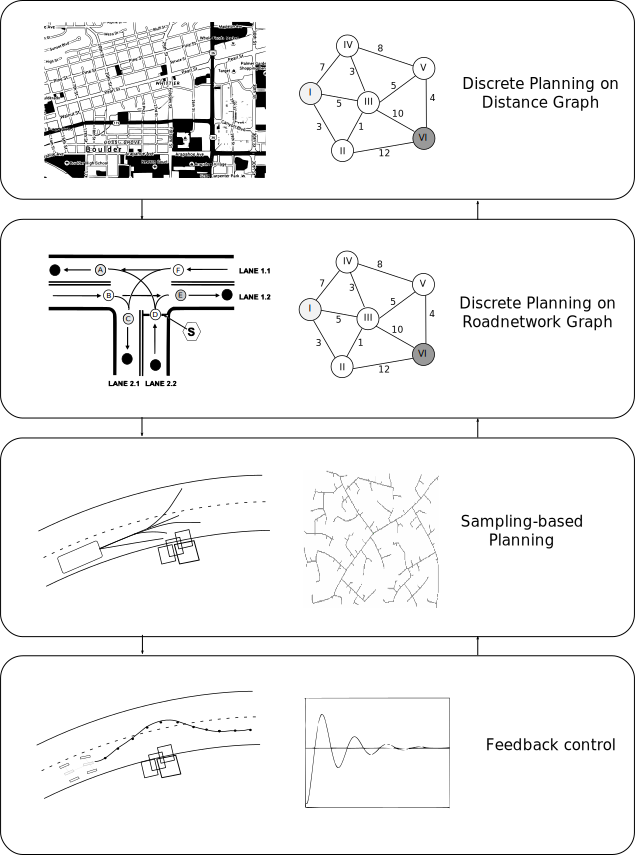
\includegraphics[width=0.9\textwidth]{figs/planninglayers}
% \caption{Path-planning across different length scales, requiring a variety of map representations and planning paradigms. Arrows indicate information passed between layers.\label{fig:planninglayers}}
\caption{不同长度尺度的路径规划,需要各种地图表示和规划范例。箭头表示层之间传递的信息。
\label{fig:planninglayers}}
\end{figure}

% Note that this representation does not include a reasoning level that encodes traffic rules and common sense. While some of these might be encoded using cost-functions, such as maximizing distance from obstacles or insuring smooth riding, other more complex behaviors such as adapting driving in the presence of cyclists or properties of the ground need to be implemented in an additional vertical layer that has access to all planning layers. 

请注意,此表示不包括编码流量规则和常识的推理级别。虽然其中一些可能使用成本函数进行编码,例如最大化与障碍物的距离或确保平稳骑行,但是还需要在附加垂直层中实施其他更复杂的行为,例如在骑自行车者或地面性质的情况下适应驾驶 可以访问所有规划层。


% \section{Other path-planning applications}
% Once the environment has been discretized into a graph, we can employ other algorithms from graph theory to plan desirable robot trajectories. For example, floor coverage can be achieved by performing a depth-first search (DFS) or a breadth-first-search (BFS) on a graph where each vertex has the size of the coverage tool of the robot. ``Coverage'' is not only interesting for cleaning a floor: the same algorithms can be used to perform an exhaustive search of a configuration space, such as in the example shown in Figure \ref{fig:inversekinematics}, where we plotted the error of a manipulator arm in reaching a desired position over its configuration space. Finding a minimum in this plot using an exhaustive search solves the inverse kinematics problem. Similarly, the same algorithm can be used to systematically follow all links on a website till a desired depth (or actually retrieving the entire world-wide web).

\section{其他路径规划应用程序}
一旦将环境离散成图,我们可以使用图论中的其他算法来规划所需的机器人轨迹。例如,可以通过在每个顶点具有机器人的覆盖工具的大小的图上执行深度优先搜索(DFS)或宽度优先搜索(BFS)来实现层覆盖。“覆盖”不仅对清理底板感兴趣:可以使用相同的算法来对配置空间进行详尽的搜索,例如在图\ref{fig:inversekinematics}中所示的示例中,我们绘制了操纵臂在其配置空间上达到所需位置的误差。使用详尽的搜索在该图中找到最小值可以解决逆运动学问题。类似地,可以使用相同的算法来系统地跟踪网站上的所有链接,直到所需的深度(或实际检索整个全球网络)。

% Doing a DFS or a BFS might generate efficient coverage paths, but they are far from optimal as many vertices might be visited twice. A path that connects all vertices in a graph but passes every vertex only once is known as a \emph{Hamiltonian Path}.\index{Hamiltonian Path} A Hamiltonian path that returns to its starting vertex is known as a Hamiltonian Cycle. This problem is also known as the Traveling Salesman Problem (TSP), in which a route needs to be calculated that visits every city on his tour only once and is known to be NP Complete.\index{Traveling Salesman Problem}

执行DFS或BFS可能会生成有效的覆盖路径,但是它们远不是最佳的,因为可能会访问两个顶点。连接图中所有顶点但仅将每个顶点仅传递一次的路径称为\emph{Hamiltonian Path}\index{Hamiltonian Path}返回到其起始顶点的哈密尔顿路径被称为哈密尔顿循环。这个问题也被称为旅行推销员问题(TSP),其中需要计算一次路线访问他的旅程中的每个城市一次,并且被称为NP完成。\index{旅行推销员问题}

% \section{Summary and Outlook}
% Path planning is an ongoing research problem. Finding collision free paths for mechanisms with high degrees of freedom such as multiple arms operating in a common space, multi-robot systems, or systems involving dynamics (and therefore adding the derivatives of the state variables to the planning problem) might take unacceptably long to solve.
 
\section{总结和展望}
路径规划是一个持续的研究课题。寻找具有高度自由度的机制的无碰撞路径,例如在公共空间中操作的多臂,多机器人系统或涉及动力学的系统(并因此将状态变量的导数添加到规划问题)可能需要不可接受的长时间解决。

% Although sampling-based path planners can drastically speed up the time to find some solution, there are not optimal and struggle with specific situations such as narrow passages. There is no ``silver bullet'' algorithm for solving all path planning problems and heuristics that lead to massive speed-up in one scenario might be detrimental in others. Also, algorithmic parameters are mostly ad-hoc and correctly tuning them to a specific environment might drastically increase performance.

虽然基于采样的路径规划者可以大大加快找到解决方案的时间,但是对于具体的情况,如狭窄的段落,并不是最佳的。没有一种用于解决所有路径规划问题的“子弹”算法,导致在一种情况下大规模加速的启发式算法在其他情况下可能是有害的。此外,算法参数大多是特别的,并且正确地将它们调整到特定环境可能会大大提高性能。


% \section*{Take-home lessons}
\section*{课后补充}
\begin{itemize}
% \item The first step in path planning is choosing a map representation that is appropriate to the application.
% \item The second step is to reduce the robot to a point-mass, which allows planning in the configuration space.
% \item This allows the application of generic shortest path finding algorithms, which have applications in a large variety of domains, not limited to robotics.
% \item A sampling-based planning algorithm finds paths by sampling random points in the environment. Heuristics are used to maximize the exploration of space and bias the direction of search. This makes these algorithms fast, but neither optimal nor complete.
% \item As the resulting paths are random, multiple trials might lead to totally different results.
% \item There is no one-size-fits-all algorithm for a path-planning algorithm and care must be taken to select the right paradigm (single-query vs. multi-query), heuristics, and parameters.

\item 路径规划的第一步是选择适合应用程序的地图表示。
\item 第二步是将机器人减少到一个点 - 质量,这允许在配置空间中进行规划。
\item 这允许应用通用的最短路径查找算法,它们在各种各样的域中都有应用,不仅限于机器人。
\item 基于抽样的规划算法通过对环境中的随机点进行抽样来找到路径。 启发式用于最大限度地探索空间并偏向搜索方向。 这使得这些算法快速,但既不是最优也不完整。
\item 由于生成的路径是随机的,多次试验可能会导致完全不同的结果。
\item 对于路径规划算法,没有一个适合所有算法的算法,必须注意选择正确的范例(单查询与多查询),启发式和参数。
\end{itemize}

% \section*{Exercises}\small
\section*{习题}\small
\begin{enumerate}
% \item How does the computational complexity of Dijkstra's algorithm change when moving from 2D to 3D search spaces?
% \item A* uses a ``heuristic'' to bias the search in the expected direction of the goal. Why can it only use a heuristic, not the actual length?
% \item Assuming points are sampled uniformly at random in a randomized planning algorithm. Calculate the limiting behaviour of the following ratio   (number of points in tree)/(number of points sampled) as the number of points sampled goes to infinity. Assume the total area $A_{total}$ and the area of free space $A_{free}$ within are known. 

% \item Assuming a kd-tree is used as a nearest-neighbour data structure, and points are sample uniformly at random, calculate the  run-time of inserting a point into a tree of size $N$. Use ``big-Oh'' notation, e.g. $\mathcal{O}(N)$.

% \item What other practical runtime concerns must one consider besides computational complexity alone when doing sampling based motion planning? Can you suggest ways to deal with these other concerns?

\item 从2D到3D搜索空间移动时,Dijkstra算法的计算复杂度如何变化?
\item A*使用“启发式”来将搜索偏向目标的预期方向。为什么只能使用启发式,而不是实际的长度?
\item 假设点在随机规划算法中随机抽样。当采样点数达到无穷大时,计算以下比例(树中的点数)/(采样点数)的限制行为。假设总面积$A_{total}$和可用空间面积$A_{free}$已知。

\item 假设使用kd-tree作为最近邻数据结构,并且点随机抽样,计算将点插入到大小为$N$的树中的运行时间。使用“大哦”表示法,例如$\mathcal{Ó}(N)$。

\item 在进行基于抽样的运动规划时,除了计算复杂度之外,还有哪些实际运行时问题必须考虑?你能建议处理这些其他问题的方法吗?

\end{enumerate}

\normalsize